\input{./UCLHeader.tex}
%New commands
%Maths
\newcommand{\beq}{\begin{equation}}
\newcommand{\eeq}{\end{equation}}
\newcommand{\bea}{\begin{align}}
\newcommand{\eea}{\end{align}}
\newcommand{\p}{\partial}
\newcommand{\trace}[1]{\mathrm{Tr}\left[#1 \right]}
\newcommand{\ptrace}[2]{\mathrm{Tr}_{#1} \left[ #2 \right]}
\newcommand{\bpmat}{\begin{pmatrix}}
\newcommand{\epmat}{\end{pmatrix}}
\newcommand{\vv}[1]{\vec{#1}}
\newcommand{\mat}[1]{\uuline{#1}}
\newcommand{\norm}[1]{\| #1 \|}
\newcommand{\op}[1]{\mathbb{#1}}
\newcommand{\vhat}[1]{\hat{\vv{#1}}}


%Renewed commands, in order for them to take arguments with automatically adjusted brackets 
\renewcommand{\dim}[1]{\mathrm{dim}\left( #1\right)}
\renewcommand{\det}[1]{\mathrm{det} \left( #1 \right)}
\renewcommand{\exp}[1] {\mathrm{exp} \left[ #1 \right]}


%\mathbb Letters
\newcommand{\identity}{\mathbb{I}}
\newcommand{\inreal}{\mathbb{R}}
\newcommand{\incomplex}{\mathbb{C}}

%Redefine Braket
\renewcommand{\braket}[1]{\left\langle #1 \right\rangle}

%Integration
\newcommand{\intd} {\mathrm{d}}

%Operators
\newcommand{\phihat}{\hat{\phi}}
\newcommand{\xhat}{\hat{x}}
\newcommand{\phat}{\hat{p}}
\newcommand{\Dhat}{\hat{D}}
\newcommand{\Hhat}{\hat{H}}
\newcommand{\ahat}{\hat{a}}
\newcommand{\bhat}{\hat{b}}
\newcommand{\chat}{\hat{c}}
\newcommand{\Phihat}{\hat{\Phi}}

%Channels
\newcommand{\channel}[3]{\mathcal{#1}^{#2 \rightarrow #3}}


%Caligraphy letters
\newcommand{\cl}[1]{\mathcal{#1}}
\newcommand{\Hilbert}{\mathcal{H}}
\newcommand{\calN}{\mathcal{N}}
\newcommand{\Lag}{\mathcal{L}}
\newcommand{\calD}{\mathcal{D}}


%Pauli
\newcommand{\Xhat}{\hat{X}}
\newcommand{\Yhat}{\hat{Y}}
\newcommand{\Zhat}{\hat{Z}}
\newcommand{\PauliX}{\bpmat 0 & 1 \\ 1 & 0 \epmat}
\newcommand{\PauliZ} {\bpmat 1 & 0 \\ 0 & -1\epmat}



%Gell-Mann matrices
\newcommand{\GMone} {\bpmat 0 & 1 & 0 \\ 1 & 0 & 0 \\ 0 & 0 & 0 \epmat }
\newcommand{\GMsix}{\bpmat 0 & 0 & 0 \\ 0 & 0 & 1\\ 0 & 1 & 0\epmat}

%Density matrices
\newcommand{\rhotwo}{\bpmat 1 & e^{-it} \\ e^{it} & 1 \epmat}
\newcommand{\rhothree} {\bpmat 1 & e^{it} & e^{2it} \\
e^{-it} & 1 & e^{it} \\
e^{-2it} & e^{-it} & 1 \epmat}



%Misc
\def\dbar{{\mathchar'26\mkern-12mu d}} %a $d$ with a bar through its stem


\newcommand{\eq}[1]{$#1$}

%Undertilded quantities
\newcommand{\tildeq}{\underset{^\sim}q}
\newcommand{\tildep}{\underset{^\sim}p}

%Curly letters
\newcommand{\calE}{\mathcal{E}}

\newcommand{\Nhat}{\hat{N}}

%Wave vector shortening
\newcommand{\kvec}{\vv{k}}

%Change braket size in ket and bra commands
\renewcommand{\ket}[1]{\left| #1 \right\rangle}
\renewcommand{\bra}[1] {\left\langle #1 \right|}












\begin{document}
\title{Superconductivity Long Notes}
\author{Sofia Qvarfort}
\maketitle
\tableofcontents

\section{Superconductivity}
\subsection{Introduction}
\begin{description}
\item[Requirements for macroscopic quantum phenomena] are
\begin{itemize}
\item Sufficiently low temperatures
\item Particles must `notice' that they are indistinguishable 
\item Non-localisation 
\end{itemize}

\item[Regime for BEC behaviour] holds when the Compton wavelength is similar to the interparticle distance. 
\beq
\lambda \geq n^{-1/3}
\eeq
In thermal equilibrium, we find
\beq
p \sim \left( mk_B T\right)^{1/2}
\eeq
and thus we require
\beq
k_B T \leq \frac{n^{2/3}  \hbar^2}{m}
\eeq
where $m$ is the particle mass. 
Especially for heavy atoms, this means that the temperatures have to be sufficiently low. 

\item[Candidate systems] include
\begin{itemize}
\item some atoms or molecules
\item Liquid  He-3 or He-4
\item Dilute atomic alkali gases
\item Electrons in metals
\item Quasiparticles, such as excitons, polarisons and magnons
\item Photons interacting via coupling to some matter component
\end{itemize}


\end{description}

\subsection{Bosons: BEC Basics}
\begin{description}
\item[Simple definition] A BEC is a system that is in one single macroscopic state. For a wavefunction
\beq
\psi_s(r_1, r2, \ldots r_N)
\eeq
which is symmetric exchange, we get the density matrix
\beq
\rho(r, r') = N \sum_s p_s \int \intd r_2 \intd r_3 \ldots \int r_N \Psi^*_s(r, r_2, \ldots , r_N) \Psi_s(r', r_2 , \ldots , r_N)
\eeq
This is just the inner product of $\braket{\psi^\dagger(r) \psi(r')}$. where I guess that $\psi(r)$ is a single-particle wavefunction. If we diagonalise, we get
\beq
\rho(r, r') = \sum_j n_j \chi^*_j (r) \chi_j(r')
\eeq
Once one of the eigenvalues dominate, we say that we are in a macroscopic state. 


\item[Infinite and translationally invariant systems] gives a single-particle wavefunction 
\beq
\chi_j(r) = e^{i \vv{k}_j \cdot \vv{r}/\sqrt{V}}
\eeq

\item[Macroscopic eigenvalue] $N_0$ for the $\chi_j(r)$ wavefunction given by 
\beq
\lim_{|r- r'|\rightarrow \infty} \rho(r, r') = \frac{N_0}{V}
\eeq
Question: If we are dealing with an infinite system, should not $V \rightarrow \infty$?

\end{description}
\subsection{Non-interacting Bose gas}
\begin{description}
\item[Statistics] for bosons is given by 
\beq
n_k = 	\frac{1}{e^{\beta( \epsilon_k - \mu)} - 1}
\eeq
where
\beq
\epsilon_k = \frac{\hbar^2 k^2}{2m}
\eeq
is the energy of a free particle, and where $\mu$ is the chemical potential. 

\item[Chemical potential] often written $\mu$ is the amount of energy required to add another paticle to the system. 

\item[Total number of particles] given by integrating over all energies, 
\beq
N = \int \intd \epsilon \frac{g(\epsilon)}{e^{\beta(\epsilon_k - \mu)} - 1}
\eeq
where
\beq
g(\epsilon) \propto \epsilon^{d/2 - 1}
\eeq
is the density of states. 

Question: I can't recall how the dimensionality of space comes into this. 

Answer: We are concerned with the \emph{density of states}, which necessarily is related to the dimensionality as we ask the question how many states we can fit in per unit volume. 

\item[Requirement for well-defined $n_k$] is 
\beq
\mu \leq 0
\eeq

\item[Maximum number of particles]  the largest possible value of $\mu$ is $\mu = 0$, thus
\beq
N_{max} = \int \intd \epsilon \frac{\sqrt{\epsilon }}{e^{\beta \epsilon _k } - 1}
\eeq
If we add more particles, we cannot describe the statistics by the Bose-Einstein distribution anymore. 

\item[Macroscopic occupancy] instead, while we are below $T_c$, any new addition will occupy a single state
\beq
N = N_0+ N_{max}
\eeq

Question: I thought we were talking about states and not number. However, could this be that below the temperature, we just treat the new particles as one single particle? 



\end{description}
\subsection{Weakly interacting dilute Bose gas}
\begin{description}
\item[Full Hamiltonian] is given by 
\beq
H = \sum^N_{i = 1} \left[- \frac{\hbar \nabla^2_i}{2m} + V(r_i)\right] + \sum_{i < j} U\delta (r_i - r_j) 
\eeq

\item[Variational Principle] is the way of finding the minimum energy. We start with a guess for a ground state, then work out the energy. From there, we look at which parameters go into the wavefunction, the minimise the energy from there. 

In the context of superconductivity, the variational principle can be used to find the ground state by minimising the free energy $F$. 

\item[Free energy] is given by
\beq
F = N \int  \intd^3 r \left[ \frac{\hbar^2 }{2m } |\nabla \chi|^2 + \left( V(r) - \mu \right) |\chi|^2 + \frac{UN(N-1)}{2} |\chi|^4 \right]
\eeq

\item[Derivation of the Gross-Pitaevskii equation] We wish to derive the equation of motion for the system with the potential above by minimising the free energy. First, we rescale the wavefunction 
\beq
\chi = \sqrt{N} \psi(r)
\eeq
We obtain
\beq
F = \int \intd^3 r \left[ \frac{\hbar^2}{2m} |\nabla^2\psi^2| + \left( V(r) - \mu \right) + \frac{U(N-1)}{2} |\psi|^4 \right]
\eeq
This quantity is at its minimum where the derivative of the quantity inside the integral is zero. Differentiating with respect to $\psi$ gives
\beq
\frac{\hbar^2}{2m} \nabla^2 \psi + \left( V(r) - \mu\right) |\psi|^2  + U(N+1) |\psi|^3 = 0
\eeq
This is a bit like a non-linear Schrodinger equation. 

\item[Chemical potential for translationary invariant systems] A translationary invariant system has, 
\beq
\psi = \sqrt{\frac{N}{V}}
\eeq
then solving the Gross-Pitaevskii is given by 
\beq
\mu = \frac{UN}{V}
\eeq


\item[Time dependent Gross-Pitaevskii equation] we can combine the above with the TDSE to get
\beq
i \hbar \frac{d \psi(r,t)}{dt} = \left[- \frac{\hbar^2 \nabla^2}{2m} + V(r) + U|\psi(r, t)|^2 \right] \psi(r,t)
\eeq

\item[BEC ground state] is characterised by its average number of particles. It can be either a state with well-defined particle number or well-defined phase. 
\beq
\ket{\Psi_N} = \left( \psi^\dagger_0\right)^N \ket{\Omega}
\eeq
\beq
\ket{\Psi_\lambda} = e^{\lambda \psi^\dagger_0 - |\lambda|^2/2 } \ket{\Omega}
\eeq
The first one is a Fock state and the second is a coherent state. The coherent state has lower energy, and thus the ground state does not have well-defined particle number. 

\end{description}
\subsection{Fragmented BEC}
\begin{description}
\item[Fragmented BEC] for two closely separated states $\chi_0$ and $\chi_1$ can be described by 
\beq
\ket{\Psi} = \left( \psi^\dagger_0 \right)^{N-M} \left( \psi^\dagger_1 \right)^M \ket{\Omega}
\eeq

\item[Interaction energy difference] given by 
\beq
\frac{U}{2V} \left( ( N-M)(N-M-1) + M(M-1) + 4(N-M)M \right) \simeq \frac{U}{2V} \left[ N^2 + 2M(N-M) \right] \nonumber
\eeq
We have made the approximation of removing one $N$ from the expression above. 


\end{description}

\subsection{Fluctuations}
\begin{description}
\item[Guassian state] is given by
\beq
\psi(r) = \frac{1}{\sqrt{V}} \sum_k \psi_k e^{i \vv{k} \cdot \vv{r}} 
\eeq

\item[BEC Hamiltonian] the Hamiltonian for the weakly interacting gas is, in 2nd quantisation, 
\beq
H - \mu N = \sum_k ( \epsilon_k - \mu )  \psi_k^\dagger \psi_k + \sum_{k , k', q} \frac{U}{2V} \psi^\dagger_{k + q} \psi^\dagger_{k'- q} \psi_{k'} \psi_k
\eeq


\item[Quasi-particle Hamiltonian] the previous Hamiltonian can be diagonalised into 
\beq
H = \sum_k \xi_k b_k^\dagger b_k + \frac{\xi_k - \epsilon_k - \mu}{2}
\eeq

\item[Boboliubov transformation] is a unitary transformation of a commutator relation, such as $[a, a^\dagger] = 1$. Note that in addition to the hyperbolic transformation matrix, we can also add a phase $e^{i \theta}$ to the transformation, since this will be cancelled out. 

\item[More stuff needed here]



\end{description}

\subsection{Fermions - BCS-BEC Crossover}
\begin{description}
\item[BCS theor] describes bonding between fermions and can explain most superconductors. BCS works well when
\begin{itemize}
\item Transitions temperatures must be a small fraction of the Fermi degeneracy temperature $T_F$
\item Normal state is of a normal metal 
\item Superconductor transition does not occur close to an additional phase transition 
\item The symmetry of the Cooper pairs is the same as the crystal lattice or $s$-wave in the case of amorphous materials
\item The principal mechanism of Cooper pairing is the exchange of virtual phonons
\end{itemize}

\item[Fermi Temperature] written $T_F$ is defined as
\beq
T_F = \frac{E_F}{k_B}
\eeq
where $E_F$  is the Fermi energy.  $T_F$ is the temperature at which thermal effects are comparable with quantum efects associated with Fermi statistics. 

\item[Virtual phonons] are needed to describe static lattice deformations surrounding a perturbation. They are a field/theoretical tool  required for the transfer of forces and such. 

\item[Cooper problem] phonon cause a weak attraction between the electrons. 

\item[Cooper pairs] are pairs of electrons with momentum with $\ket{k}$ and $-\ket{k}$. Only a few electrons close to the Fermi energy get paired. A Cooper pair is of bosonic nature since it is made up of an even number of fermions. 

Each electron has spin-1/2, which when added can have either spin 1 or spin 0. 

\item[Pairing instability] is based on seeing the superconducting transition as an instabilityof the normal state at some finite temperature. It highlights the potential importance of pairing fluctuations that occur in the normal state even before the critical transition. 

\item[BCS instability] not entirely sure what this is. I think it is adding an instability to the BEC treatment that we performed before. 

\end{description}
\subsection{Fermion ground-state wavefunction}
\begin{description}
\item[Initial assumptions] we assume that a number of $N$ electrons in an alkali metal will have $N/2$ be in the spin-up state and $N/2$ be in the spin-down state. The electrons are moving in  a free 3D space subject to attractive interactions. 

\item[BCS postulate] the ground state is a condensate of a macroscopic number of fermion pairs. Any two different species of particles form a singlet. 

\item[BCS ground state] is given by 
\beq
\Psi_N = \mathcal{A} \left\{\varphi|(\vv{r}_1 - \vv{r}_2|  ) \chi_{12} \ldots \phi(|\vv{r}_{N-1} - \vv{r}_N |)\chi_{N-1, N}\right\}
\eeq
$\mathcal{A}$ is an operator that anti-symmetrises for any exchange of coordinates or spins for any of the electrons. 

\item[BCS ground state] in second quantisation is also written 
\beq
\ket{\Psi}_N = \int \prod_i \intd ^3 r_i \varphi(\vv{r}_1 - \vv{r}_2)\Psi^\dagger_{\uparrow} (\vv{r}_1) \Psi^\dagger_{\downarrow} (\vv{r}_2)\ldots \varphi(\vv{r}_{N-1} - \vv{r}_N) \Psi^\dagger_{\uparrow} ( \vv{r}_{N-1}) \Psi^\dagger_{\downarrow} (\vv{r}_N) \ket{0}
\eeq

Or, more succinctly, 
\beq
\ket{\Psi}_N = (b^\dagger)^{N/2} \ket{0}
\eeq


\item[Field operator] lol... is given by 
\beq
\Psi^\dagger_\sigma ( \vv{r}) = \sum_k c^\dagger_{k \sigma} \frac{e^{- i \vv{k}\cdot \vv{r}}}{\sqrt{V}}
\eeq

\item[Creation operator for Fermion pair]  given by 
\beq
b^\dagger = \sum_k \varphi_k v_{k \uparrow} ^\dagger c^\dagger_{- k \downarrow}
\eeq


\end{description}
\subsection{Superfluidity}
\begin{description}
\item[Superfluid wavefunction] is macroscopic and complex, and is given by 
\beq
\psi( \vv{r}) = |\psi(\vv{r})| e^{i \phi(\vv{r})}
\eeq

Note: This is a solution to the Gross-Pitaevskii equation for a condensate in a macroscopic cylinder. 

\item[Current operator] given by 
\beq
\vv{J}(r) = \frac{\hbar}{2m*i} \left[ \psi^\dagger( r) \vv{\nabla} \psi(r) - \psi(r) \nabla \psi^\dagger(r) \right]
\eeq

\item[Superfluid velocity] is the gradient of the phase, 
\beq
\vv{v} = \frac{\vv{J}}{density} = \frac{\hbar}{m*} \vv{\nabla} \phi
\eeq
which we can show if we write out the expression for the current. The requirements for this to hold are: the wavefunction amplitude $|\psi(\vv{r})|$ must (as in this case) be Hermitian, and the phase $\phi(\vv{r})$ must depend on the position of the superfluid. Note that his makes the phase a local phase, and not global. 

Question: When I calculate the current, I get exactly $\frac{\hbar}{m*} \vv{\nabla} \phi$. Where does the density come into this? 

Attempt at answer: I think that $\vv{J}$ might in the first case actually be the current density. 

\item[Consequence of superfluid velocity] the curl of a gradient is always zero. Thus
\beq
\vv{\nabla} \times \vv{v} = \vv{\nabla} \times \frac{\hbar}{m*} \vv{\nabla} \phi = 0
\eeq
For proof, just write the whole thing out and remember that partial derivatives commute. 

Consequence: The superfluid is \emph{irrotational}. 

\item[Mass of fermionic superfluids] is $m* = 2m$ because we are dealing with Cooper pairs. 

\item[Circulation] is the line integral around a closed curve of a velocity field. It is written
\beq
\Gamma = \oint_C \vv{v} \cdot \intd \vv{l}
\eeq
Essentially, it is a useful wauntity in hydrodynamics that helps us deal with various scenarios. 


\item[Vortex derivation] As we start rotating the cylinder that contains the superfluid, the superfluid can remain stationary until we increase the angular velocity $\Omega$ to a certain point. A stationary liquid in a rotating container has high free energy (why?) thus at some point it is beneficial for the superfluid to introduce vortices. 

Note that whenever we speak about a vortex, we speak about \emph{probability waves}! 

We know that if we walk around the condensate and return to the same point, the uniqueness (single-valuedness) of the wavefunction requires that the phase $\phi$ changes by and integer $n $ of $2\pi$. Therefore, if we try and calculate the circulation of the fluid, we find
\beq
\Gamma = \oint_C \vv{v} \cdot \intd \vv{l} 
\eeq
Now, the vector $\vv{r}$ is a general displacement vector. If we confine the contour $C$ to a 2D plane, we can limit ourselves to a 2D geometry in polar coordinates. Then, we find
\beq
\vv{\nabla} = \frac{\p }{\p r} + \frac{1}{r} \frac{\p}{\p \theta}
\eeq
where $\theta$ is the angle we are walking around. Subsequently, the quantum phase $\phi(\vv{r})$ is now a function of radius $r$ and angle $\theta$ in some plane. We also find that 
\beq
\intd \vv{l} = r \intd \theta \vhat{\theta}
\eeq
This in turn means that 
\begin{align}
\oint_C \vv{v} \cdot \intd \vv{v} &= \frac{\hbar}{m*} \oint \left( \frac{\p \phi(r, \theta)}{\p r} \vhat{r}+ \frac{1}{r} \frac{\p \phi(r ,\theta)}{\p \theta}\vhat{\theta} \right) \cdot r \intd \vv{\theta}  \\
&= \frac{\hbar}{m^*} \oint \frac{\p \phi(r, \theta)}{\p \theta} \intd \theta \\
&= \frac{\hbar}{m^*} \left( \phi(r, 2\pi) - \phi(r, 0) \right) \\
&= \frac{\hbar}{m^*} 2\pi n \\
&= \frac{h}{m^*}n
\end{align}
This equation satisfies the situation where we have zero circulation, $\Gamma = 0$ which occurs for $n = 0$. However, we can also have finite circulation, which corresponds to irrotational vertices (with zero curl). \emph{The circulation is quantised}. 


Thus, whereas the overall curl of the liquid $\vv{\nabla} \times \vv{v} 
 $ must be zero, there can still be a local non-zero $\vv{v}$. For $\vv{v}$ to be non-zero, we require a change in $\phi$. When we have a vortex, there has been a change in $\phi$. In a 2D plane, this occurs at a single point (the axis of the vortex). However, since we can't have a discontinuous flux (which means that $\vv{\nabla} \phi$ would go to infinity, we require that the \emph{density} at that point also goes to infinity. That is, we know that 
\beq
I = n v
\eeq
The current must remain finite (maybe some kind of current conservation argument?) and therefore the density has to compensate for the velocity diverging. 


 
\item[Irrotational vortex] A particle trapped in this vortex will go around the vortex, but will not spin. Therefore, this vortex will have no curl. Any particle trapped within the vortex will follow horizontal flow lines. If we know the circulation of the irrotational vortex, we can infer some other physical quantities. 

The tangential component of the probability wave velocity around the vortex is
\beq
u_\theta = \frac{\Gamma}{2\pi}
\eeq
and the angular momentum per unit mass relative to the vortex axis is therefore constant
\beq
ru_\theta = \frac{\Gamma}{2\pi}
\eeq
This is how a superfluid can carry angular momentum. 

\end{description}
\subsubsection{Landau criterion for superfluidity}
\begin{description}

\item[Landau criterion] states that there exists a maximum velocity above which the fluid flow becomes dissipative and loses its superfluid nature. 

\item[Landau criterion derivation] Consider a superfluid with velocity $\vv{v}$ relative to some container. We create an excitation in the superfluid of momentum $\hbar \vv{k}$. This can be done by introducing an obstacle or similar. 

In the lab rest frame, creating this excitation costs the potential and kinetic energy given by 
\beq
E_k + \hbar \vv{k} \cdot \vv{v}
\eeq
The second term is the kinetic energy, since $\hbar \vv{k}$ is a momentum. The expression is minimised for momenta with negative $\vv{k}$ relative to $\vv{v}$. For large enough $k$, the cost of the excitation is negative, and therefore favourable. 

Thus, for any $k$, the critical velocity is given by 
\beq
v_c = \min_{k} \frac{E_k}{\hbar k}
\eeq
The nature of $k$ depends on the excitation. 

\item[Critical velocity in BCS limit] is given by
\beq
v_{c, BCS} = \frac{\Delta}{\hbar k_F}
\eeq
where $\Delta$ is the superconductor gap. 

\item[Critical velocity interpretation] when an object moves through the superfluid faster than $v_c$, it will break Cooper pairs. For BECs however, where we deal with tightly bound bosons, we require more energy and so those liquids are usually stabler. Thus for large $k$
\beq
v_{c, BEC} = ck
\eeq
where $c$ is the speed of sound. 

\end{description}
\subsubsection{Superfluid response functions}
\begin{description}
\item[Redefinition of superfluid] The Landau criterion doesn't apply to complex spectra. Thus, we define the superfluid density is defined in terms of linear response theory. 

\item[Response function] written $\chi_{ij}(q)$ determines what value the current $J_i(q)$ takes from a small perturbation $f(q)$ where $q$ is momentum. That is, the response function maps linear perturbations onto a current. The curent is given by 
\beq
J_i(q) = \sum_k \frac{k_i}{m} \psi^\dagger_{k + q/2} \psi_{k - q/2}
\eeq

\item[General $\chi_{ij}$ for isotropic system] in the limit of $q \rightarrow 0$ is 
\beq
\chi_{ij}(q) = \chi_T\left( \delta_{ij} - \frac{q_i q_j}{q^2} \right) + \chi_L \frac{q_i q_j}{q^2}
\eeq


\item[Superfluid part] given by 
\beq
\chi_S = \chi_L - \chi_T
\eeq


\end{description}

\subsection{Experimental systems}
\begin{description}
\item[Ultracold alkali gases] Alkali gases can be lasercooled to near 0K. This enables them to form superfluids. Through the hyperfine interaction, we can manipulate the interaction properties of the atoms through Feshback resonance via magnetic fields. 

\item[Feshback resonance] is achieved when one internal degree of freedom for a many-body system disappears. It occurs when the energy of a bound state of an interacomit potential is equal to the kinetic energy of a colliding pair of atoms. 


\end{description}
\subsubsection{Excitons and Polaritons}
\begin{description}
\item[Temperature-mass relationship] We know that
\beq
T \propto \frac{1}{m}
\eeq
Therefore, light particles don't need very low temperatures, which makes them good candidates. 

\item[Excitons] are  bound pairs of electrons and holes. 

\item[Exciton Hamiltonian] given by 
\beq
H = E_g  - \frac{\hbar^2 \nabla^2_e}{2m_c} - \frac{\hbar^2 \nabla^2_h}{2m_v} - \frac{e^2}{4 \pi \epsilon |r_e - r_h|}
\eeq
The last term is a Coulomb interaction. This has hydrogen-like solutions. 

Question:  what are $m_c$ and $m_v$? 

Attempt at answer: Could it be that since we are dealing with electrons in either the conduction band or valence band (since we are in a alkali metal which has bands) that the masses refer to the electrons in respective bands? Maybe this is the case, but they don't usually have different mass, do they? 


\item[Hamiltonian for many excitons]  near the band gap is given by 
\beq
H = \sum_k \left( \epsilon_c(k) a^\dagger_{ck} a_{ck} + \epsilon_v(k) a^\dagger_{vk} a_{vk} \right) + \frac{1}{2} \sum_q \left( V^{ee}_q \rho^e_q \rho^e_{-q}  + V^{hh}_q \rho^h_q \rho^h_{-q} - 2 V^{eh}_q \rho^e_q\rho^h_{-q} \right)
\eeq
where
\beq
\rho^e_q = \sum_k a_{ck + q}^\dagger a_{ck}
\eeq
\beq
\rho^h_q = \sum_k a_{vk-q} a^\dagger_{vk}
\eeq




\end{description}
\section{Classical Josephson Junctions}
\begin{description}
\item[Critical Temperature] called $T_C$, the temperature below which resistivity goes to zero. 

\item[Element with highest $T_C$] is niobium at $9$K. 

\item[Compound with highest $T_C$] is Mercury-Thallium-Barium-Copper-Oxide with 138 K. 

\item[Cooper pairs] are pairs of electrons which form through a mutually attractive pairing interaction. This arises through electron-phonon interactions. 

\item[Spin of electron in a Cooper pair] are always opposing because of the Pauli exclusion principle. 

\item[Meissner Effect] describes the expulsion of magnetic fields from a superconductor. The screening happens through currents appearing in the superconductor, which counter the magnetic field. The superconductor is therefore a perfect diamagnet. 

\item[Magnetic susceptibility] for a superconductor where we observe the Meissner effect is equal to 
\beq
\frac{dM}{dH} = -1
\eeq
Here, $M$ is the magnetisation of the material, which is the magnetic dipole moment per unit volume, and $H$ is the magnetic field strength. 

\item[Penetration depth] is the characteristic length scale for which the magnetic field dies down in the superconductor. The magnetic field decreases exponentially. 

\item[Destruction of superconductivity] occurs at some critical field strength $H_C$, where the material will become resistive and allow magnetic fields into its interior. 

\item[Critical current] called $J_C$ exists, above which the material becomes resistive. 

\item[Conditions for superconductivity] All quantities must be below $T_C$, $H_C$ and $J_C$ for superconductivity to occur. 

\item[Distance between Cooper pairs] can be macroscopic. Therefore, many other Cooper pairs can reside within the same area. This causes the electrons to move coherently. 

\item[Wavefunction] for electrons in a superconductor can be written down with a single pair wavefunction
\beq
\tilde{\psi}(\vv{r}) = |\psi(\vv{r})|e^{i \theta (\vv{r})}
\eeq

\item[Origin of zero resistance] is the fact that macroscopic electron pairs behave coherently. If an electron pair scatters off a phonon, the other Cooper pairs will move to compensate the phase difference. 

\item8Superconducting coherence length] usually written $\chi$, and is derived from the Cooper pair length. It can also be thought of as the characteristic exponent of the variations of density of the superconducting component. In BCS theory, it is given by 

\beq
\chi = \frac{\hbar v_f}{\pi \Delta}
\eeq
where $v_f$ is the Fermi velocity and $\Delta$ is the superconducting energy gap. 

Also, it can be found that 
\beq
\xi \propto \frac{1}{T_C}
\eeq
which is bad news for high temperature superconductors. 

One consequence of the coherence of the electrons is that we can find many quantum phenomena in superconductors, such as emulating the Young's slit experiment. 

\item[Defects] in a superconductor do not influence the behaviour as long a they are smaller than the superconducting coherence length $\xi$. 

\item[Number density of superconducting electrons] is given by the probability of detecting an electron at position $\vv{r}$, so that 
\beq
n_s( \vv{r}) = |\psi(\vv{r})|^2
\eeq

\item[Superconducting order parameter] is the absolute amplitude of the wavefucntion, $|\psi|$. It provides a measure of `how strong' the superconductivity in a sample is. It is related to the density of Cooper pairs. 

\item[Magnetic flux through superconducting loop] is \emph{quantised}. This follows from the phase coherence. Boundary conditions stipulate that the phase must differ by $2\pi$ if you go around the loop once. 

\item[Flux quantum] the minimal flux that is allowed through a superconducting loop, given by 
\beq
\phi_0 = \frac{h}{2e}
\eeq



\end{description}

\subsubsection{Type I and type II superconductors}
\begin{description}
\item[Type I superconductor] reaches its normal state immediately after the external magnetic field $H$ reaches $H_C$. 

\item[Type II superconductor] reaches its normal state gradually and not abruptly once the critical field $H_C$ has been applied. For fields below $H_C$, the magnetic flux creates discrete Abrikosov current vortices that shield the incoming field. Each vortex carries on thread of magnetic field with one flux quantum. 

As the external magnetic field increases, more and more vortices appear. Finally, the whole sample is filled with vortices, and it becomes normal (resistive) again. 

\item[Abrikosov vortex] appears in a Type II superconductor in an external field which is lower than $H_C$. A vortex can also be called a fluxon. The normal region in the vortex through which magnetic field can penetrate. 

Question: Is this just the `void' that appears in a superfluid? 

The circulating part is the current, which screens exactly one $\phi_0$. 

\item[Size of a vortex] the radius is of the scale of the penetration depth $\lambda$. We know that magnetic fields are screened on a length scale of $\lambda$, and therefore we can think of the vortex as extending over this length and shielding one flux quantum along it. 

The normal core of the vortex (where we have no shielding current) is of size $\xi$. This is because coherence can be maintained over this length scale. 

Question: I don't think I have a good, intuitive grasp on this. 

Attempt at answer: 

\item[Characterisation of Type I or Type II] we note that: \\ 
- Type I: $\frac{\lambda}{\xi} < \frac{1}{\sqrt{2}}$ \\
- Type II: all other cases. 

\end{description}
\subsubsection{The Energy Gap and Quasi Particles}
\begin{description}

\item[Energy required to break Cooper pair] is $2\Delta$. 

\item[Temperature dependence] we find that\\
- At $T = 0$ there are no phonons, just Cooper pairs \\
- At $0 < T< T_C$ there is a small but finite phonon density which can break pairs.  \\
- At $T = T_C$, all Cooper pairs have been broken \\

Note that we find that the density of Cooper pairs obeys
\beq
n \sim \frac{1}{T}
\eeq

\item[Breaking a Cooper pair] creates two quasi-particles, not electrons. A quasi-particle in a superconductor is a superposition of an electron-like particle and a hole-like particle. Resulting quasi-electrons and quasi-holes have energy $\Delta $ more than the rest of the Cooper pairs. There is an energy difference of $2\Delta$ between the `electron' and the `hole'. 

The states which above $T_C$ were within the energy gap get `pushed out' to the edge of the gap. The result is a large peak in the quasi-electron and quasi-hole densities of states at the gap edge.  

\item[Density of quasi-particle states] is given by
\beq
N_{qp} (E) = N_0 \mbox{Re} \left( \frac{E}{\sqrt{E^2 - \Delta^2}}\right)
\eeq
where $N_0$ is the single-spin density of states in the normal state. 

Question: Derivation?

\item[Electric field] causes the quasi-particles, as they move through it, they cause dissipation. At DC, the quasiparticle current is always shorted by the non-dissipative Cooper pair current. 

Question: I don't understand the last sentence. 

\item[Two-fluid model] a model for describing the conductivity of a superconductor at finite temperatures. Here, current flow is modelled as carried by $n_s$ paired electrons and $n_n$ quasi-particles. For this model, we neglect pair-breaking, by assuming that 
\beq
\frac{\omega}{2\pi} < \frac{2\Delta}{h}
\eeq

The two-fluid model attempts to explain superconductivity in e.g. liquid He below the lambda point. The components are a normal fluid and a superfluid component. Together their sum makes up the total density. 


\item[Charge conservation] the number of electrons in the normal state (above $T_C$) is given by 
\beq
n = n_s + n_n
\eeq


\item[Electric field response] the Cooper pairs move with velocity $\vv{v}_s$ and do not experience momentum-scattering collisions. The quasi-particles move with velocity $\vv{v}_n$ and experience momentum-scattering collisions at an average rate $\tau$. 

We find
\beq
2m \frac{d \vv{v}_s}{dt} = - 2e \vv{E}
\eeq
\beq
m\frac{d \vv{v}_n}{dt} = - e \vv{E} - m \frac{\vv{v}_n}{\tau}
\eeq
where $m$ is the mass of charge carriers, equal for paired electrons and quasiparticles. Note that the second term of the second equations implies a drag force. 

Question: Where does the factor of 2 in the first equation come from? 

\item[Current density ] for Cooper pairs and quasi-particles given by 

\beq
\vv{J} = - n_s e\vv{v}_s - n_n e \vv{v}_n
\eeq

\item[Conductivity] we assume that the electric field is harmonic and of the form 
\beq
\vv{E} = \vv{E}_0 e^{i \omega t}
\eeq
then we define real and imaginary conductivities from the current, 
\beq
\vv{J} = ( \sigma_1 - i \sigma_2 ) \vv{E}
\eeq
to obtain
\beq
\sigma_1 = \frac{n_n e^2 \tau}{(1 + \omega^2 \tau^2) m}
\eeq
\beq
\sigma_2 = \frac{n_s e^2 }{m \omega} + \frac{n_n e^2 (\omega \tau)^2}{(1 + \omega^2 \tau^2 ) m \omega }
\eeq

$\sigma_1$ describes the dissipative loss when a superconductor is excited by an electric field at frequency  $\omega$. It limits the Q factor of superconducting microwave resonators in Josephson qubit devices. 



Question: This needs a derivation, will get to it...



\end{description}

\subsubsection{Low $T_C$ and high $T_C$ superconductors}
\begin{description}
\item[Low $T_C$ superconductor] are metallic elemental and alloy superconductors. 

\item[High $T_C$ superconductors]  are usually made of compounds. 

\item[Differences between low $T_C$s and high $T_C$s] are the following:
\begin{itemize}
\item Pairing mechanism in low $T_C$ given by the BCS virtual phonon interaction. In high $T_C$, it is unknown. 
\item Properties of $T_C$s are anisotropic. 
\item For copper compounds, electrons that move in parallel to the cuprate planes obtain a band gap that displays four-fold symmetry. Nodes appear in the value of the gap every 90 degrees. This energy gap depends on the momentum of the paired electrons. 
\item For high $T_C$s, the properties can be tuned by doping, usually by increasing the number of oxygen atoms. 
\item The coherence length is small in high $T_C$s. It is limited by the motion of fluxons in the Lorentz force. 
\end{itemize}

Question: I presume then that the properties of low $T_C$s are generally isotropic? 


\end{description}
\subsection{Classical Properties of Josephson Junctions}
\subsubsection{Basics}
\begin{description}
\item[Josephson junction] consists of two superconducting thin films with a barrier between them. The wavefunctions $\psi_1$ and $\psi_2$ in respective section are weakly coupled. 

\item[SIS Josephson junction] is made of two superconducting thin films and an insulator. 

\item[SNS Josephson function] is made of two superconducting thin films separated by a normal metal. 


\item[Quantum behaviour] of the Josephson junction comes from the interference between the two wavefunctions
\beq
\phi = \phi_1 - \phi_2
\eeq

\item[Josephson equations] are
\beq
I_S = I_C \sin{\phi}
\eeq
\beq
V = \frac{\hbar}{2 e} \frac{\p \phi}{\p t}
\eeq
Note that $I_S$ is a supercurrent that flows through the device. This is a macroscopic quantum phenomenon. 


\item[Static solution] can be obtained when
\beq
I_S < I_C
\eeq
as we can then obtain the phase $\phi$ from the equations above. This means that $\phi$ is static, and the voltage $V$ is zero. 

\item[Unstable solution] if
\beq
I_S > I_C
\eeq
we can obtain no stable value for $\phi$ and thus $V$ is finite across the junction. 

\end{description}
\subsubsection{Resistively-Shunted junction model}

\begin{description}
\item[Contributions to the current across a Josephson junction] given by
\begin{itemize}
\item The Josephson supercurrent $I_S$ 
\item A current from the capacitance induced over a Josephson function 
\beq
I = C\frac{dV}{dt}
\eeq
\item A current formed from tunneling of quasi-particles across the junction. 
\end{itemize}

\item[Non-linear differential current equation] one can combine the above contributions to the current to write
\beq
I = I_C \sin{\phi} + \frac{\hbar} {2eR} \frac{\p \phi}{\p t} + \frac{\hbar C}{2 e} \frac{\p^2 \phi}{\p t^2}
\eeq
This can be solved numerically, but see washboard model for physical intuition. 

\end{description}
\subsubsection{Washboard model}
\begin{description}
\item[Washboard model] provides intuition about the non-linear behaviour of the supercurrent $I$ across the Josephson junction. 

\item[Washboard potential] from comparison with non-linear equation above, given by 
\beq
U(\phi) = - \frac{\hbar}{2e} \left( I_C \cos{\phi} + I \phi \right)
\eeq


\item[Rolling ball analogy] the behaviour of a ball of mass $m$ that rolls along a periodic washboard describes the dynamics pretty well. Properties:
\begin{itemize}
\item Horizontal position of ball = phase difference $\phi$
\item Viscous drag force on ball = dissipative current
\beq
F_{drag} = \frac{1}{R} \left( \frac{\hbar}{2e} \right)^2 \frac{\p \phi}{\p t}
\eeq
\item Mass of ball = proportional to capacitance $C$ of junction
\beq
m = \left( \frac{\hbar}{2e} \right)^2 C
\eeq
\item Velocity of ball = voltage across the junction
\end{itemize}

\item[Natural oscillation frequency] where the ball wiggles around in its local minima is given by 
\beq
\omega_A = \omega_P \left( 1 - \left( \frac{I}{I_C} \right)^2 \right)^{1/4}
\eeq
where $\omega_P$ is the plasma frequency. 

\item[Josephson plasma frequency] is the oscillation frequency when the net current is zero, given by 
\beq
\omega_P = \left( \frac{2 e I_C}{\hbar C} \right)^{1/2}
\eeq

Question: What here is actually oscillating? 

Attempt at answer: We said that the horizontal position of the ball is the phase difference. Therefore, it is probably the phase different that oscillates. 
\end{description}
\subsubsection{Washboard model $T= 0$}
Here we assume negligible damping. 

\begin{description}
\item[At $I = 0$] the ball is trapped in one of the minima, so
\beq
\frac{d\phi}{dt} = 0 
\eeq
which implies that $V = 0$. 

\item[Josephson energy] given by
\beq
E_J = \frac{\hbar I_C}{2e}
\eeq
where $2 E_J$ is the height of the potential barrier at $I = 0$. 

\item[Non-zero $I$] means that we have a  potential step

\beq
\Delta U\simeq 2E_J \left( 1 - \frac{I}{I_C} \right)^{3/2}
\eeq
which means that the ball can escape. With no damping, the ball keeps rolling down the washboard. 

\item[At critical current $I_C$] we see that $\Delta U = 0$. This means that 
\beq
\frac{d \phi}{dt} \neq 0
\eeq
 throughout which implies finite $V$. 
 
 \item[Below the critical current $I_C$] the ball can keep rolling. It keeps rolling until the current is reduced to zero. 
 
 \item[Hysteretic] since the ball keeps moving until $I = 0$ if we are decreasing the current, but doesn't start rolling until $I = I_C$ if increasing the current, we conclude that the system displays hysterecis. 
 
 \end{description}
 
\subsubsection{Washboard model: $T>0$ with negligible damping}
\begin{description}

\item[Brownian motion] the ball will undergo Brownian motion when it sits in the minima. The amplitude of the random walk increases with increasing $T$. This causes the ball to escape even at $I < I_C$.  The average time it takes to escape is
\beq
\tau_{TA}^{-1} = \frac{\omega_A}{2\pi} e^{- \Delta U/k_B T}  
\eeq

\item[Average number of escape attempts] per second given by $\omega_A /1 \pi$. 

\item[Switching current] written $I_{sw}$ is the value of the current at which the ball escapes by thermal fluctuation. The same $I_{sw}$ will not be found by repeating the measurement. 

\end{description}
\subsubsection{Washboard model: $T>0$ with damping}
\begin{description}
\item[Behaviour] now the ball experiences a drag force and will stop after travelling over a set number of minima. 

\item[Quality factor] called $Q$ denotes the damping in the system. It is given by 
\beq
Q = \omega_P RC
\eeq

\item[McCumber parameter] another way to measure the quality of a Josephson junction. Written
\beq
\beta_C = Q^2
\eeq


\item[Hystereic junctions] are junctions with 
\beq
Q>3
\eeq
These junctions are also known as underdamped. 

\item[Non-hysteretic junctions] have smaller $Q$ and are called overdamped. 



\end{description}

\subsection{Radio-Frequency effects in Josephson Junctions}
\begin{description}
\item[External DC voltage] which is constant means we can solve for the phase using one of the Josephson equations, 
\beq
\phi(t) = \frac{2e}{\hbar} Vt + \phi_0
\eeq
Substitute this into the first equation to get the current:
\beq
I_S = I_C \sin{\left( \frac{2e}{\hbar} Vt + \phi_0 \right)}
\eeq

\item[Supercurrent oscillation frequency] for an external voltage given by
\beq
f_J = \frac{1}{2\pi} \frac{2e}{\hbar} V
\eeq

\item[Josephson effect] is what we call the fact that the supercurrent flows across the Josephson junction. 



\end{description}
\subsubsection{Shapiro steps}
\begin{description}
\item[External RF voltage] if the voltage is no longer constant but time-dependent, $Vl(t)$, we integrate the Josephson equation to find
\begin{align}
I_S(t) &= I_C \sin{\left( \int^t_0 \frac{2e}{\hbar} v(t') \intd t' + \phi_0 \right) } \\
&= I_C \sin{\left( \frac{2eV}{\hbar} t + \frac{2eV_s}{\hbar \omega_s} \sin{\left( \omega_s t\right)} + \phi_0 \right)}
\end{align}
where $\omega_s$ is the frequency of the voltage source. 

Also note that 
\beq
v(t) = V + V_s\cos{\omega_s t}
\eeq

Question: What is the $V_s$ voltage?  

Attempt at answer: This is maximum amplitude of the oscillating voltage source. 

\item[Bessel function] are canonical solutions $y(x)$ of Bessel's differential equation:
\beq
x^2 \frac{d^2 y}{dx^2} + x \frac{dy}{dx} + (x^2 - \alpha^2 ) y = 0
\eeq
for a complex number $\alpha$. 

\item[Occurrence of Shapiro steps] current equation contains a Bessel function can be expanded to give
\beq
I_S(t) = I_C \sum_{n = - \infty}^\infty (-1)^n J_n \left( \frac{2eV_s}{\hbar \omega_s} \right) \sin{\left( (\omega_J - n \omega_s ) t + \phi_0 \right)}
\eeq

An interesting solution occurs when the source frequency is a multiple of the Josephson frequency $\omega_J = n \omega_s$. Then we see the 

\item[Shapiro steps for voltage standard] by connecting $N$ Josephson junctions together, we get very accurate Shapiro steps. They are given by 
\beq
V  = N \frac{\pi \hbar }{2} f_J
\eeq
The voltage is thus entirely determined by fundamental constants and the $f_J$, which can be precisely measured. 

\end{description}

\subsection{Josephson Junctions in a Magnetic Field}
\begin{description}
\item[Effect of $B$ field on superconducting ring ] is that we induce a phase change. Can show that 
\beq
\Delta \phi = \frac{2e}{\hbar} \int^B_A \vv{A} \cdot \intd \vv{l}
\eeq
That is, the field must be quantised. 

\item[Effect of $B$ field on Josephson junction] the total phase difference does not both depend on the difference between the two materials and the phase induced by the external magnetic field. We find
\beq
\phi = \phi_1 - \phi_2 + \frac{2e}{\hbar} \int \vv{A} \cdot \intd \vv{l}
\eeq
Note that we integrate from the interior of one of the superconducting films to the interior of the other one. 

The effect is that we can very accurately control the junction by applying an external magnetic field. 

\item[Spatially varying magnetic field] creates changes in the phase $\phi(x)$ that are in turn position dependent. We must rewrite
\beq
j_S(x) = j_c \sin{\phi (x)}
\eeq
where $j_s(x)$ is the supercurent density per unit width in the $x$ direction and $j_c$ is the  critical current density. 

\item[Calculating the total phase] we can show that (by integrating over an area inside the superconductor) that
\beq
\phi(x) - \phi(0) = 2\pi \frac{\Phi(x)}{\Phi_0}
\eeq
where
\beq
\Phi(x) = \frac{\Phi x}{w}
\eeq
and where $w$ is the width of the junction (I think). 
Question: Should $\Phi$ actually be $\Phi_0$? 
Question: I do not know what the $\Phi(x)$ term is, unless it is just a dummy variable that we have treated. 

\item[Total current under external field] is given by integrating the previous equation, 
\begin{align}
I_S &= \int^{w/2}_{- w/2} \intd x j_c \sin{\left( \phi(0) + 2 \pi \frac{\Phi(x)}{\Phi_0} \right)} \\
&= \frac{j_c w \Phi_0}{\pi \Phi} \sin{\left( \phi(0)\right)} \sin{\left( \frac{\pi \Phi}{\Phi_0} \right) }
\end{align}

\item[Maximum superurrent] that can flow through the function occurs when
\beq
\phi(0) 0 \pm \frac{\pi}{2}
\eeq
for which we obtain
\beq
I_C( \Phi) = I_c(0) \left| \frac{\sin{\left( \frac{\pi \Phi}{\Phi_0} \right) }}{\left( \frac{\pi \Phi}{\Phi_0} \right) } \right|
\eeq



\item[Critical current in zero magnetic field] is given by 
\beq
I_C(0) = j_c w
\eeq
where again $j_c$ is the critical current density and $w$ is the width of the side of the junction that runs parallel to the barrier. 

\item[Flux required to suppress critical current] is equal to one flux quantum $\phi_0$. 

Question: Is this really correct? 

Attempt at answer: Before, we said that certain superconducting properties were the same for every superconductor. However, I would have thought that we require more than one flux quantum to cancel the critical current. Although I might misunderstand. I assume that the critical current is what we whip up in order to cancel out the magnetic field. So something is wrong here. 

\end{description}

\section{Fabrication and measurement of Josephson junctions}
\subsection{Fabrication of low $T_C$ Josephson junctions}
\begin{description}
\item[Double-angle shadow evaporation] of aluminium films with aluminium oxide barriers exploits that evaporated Al atoms will travel in a straight line from the source to the substrate. Some of the substrate is protected by a mask through which the deposition is made. The mask is a suspended bi-layer resist mask fabricated using either photolithography or EBL. 

The procedure is as follows:
\begin{itemize}
\item Apply the mask
\item Evaporate the first Al layer onto the substrate
\item Allow oxygen into chamber of oxidise the Al
\item Rotate sample
\item Evaporate other side of Al
\end{itemize}


\item[`Whole wafer' Niobium Trilayer Junctions] Evaporating Nb is impossible due to its high melting point. Therefore, we grow Nb by sputter deposition. Sputter deposition is done by accelerating argon ions towards a Nb target so that Nb atoms are emitted and form a film on a nearby substrate. Nb atoms will not travel in straight line because there is Argon in the chamber. Then, the AlO layer is grown on it without breaking vacuum. 


\end{description}


\subsection{Measurement of Josephson junctions}
\begin{description}
\item[Typical measurement] consists of controlling an external magnetic field and current while measuring the ingoing and outgoing current. It has to be done in cryogenic temperatures for the junction to remain superconducting. 

\item[Shielding] the junctions must be shielded from stray electromagnetic fields (earth of mains) and from RF interference. 

\item[DC wiring to junction] is done with twisted pairs (to cancel picked-up RF on both lines) or with mini coaxial cables. A coaxial cable has an inner conductor surrounded by a tubular insulating layer, surrounded by a tubular conducting shield. 

\item[Minimising RF coupling] apart from coaxial cables and twisted pairs, we also add low temperature powder filters. 

\item[Current bias] the junctions are usually current biased because they have very low resistance. 

\item[Four terminal configuration] is used so that the potential difference across the wiring of the sample and any contact resistance is not measured. 

\item[Cryo-CMOS] amplifiers don't work at the temperatures where Josephson junctions operate. Therefore, we need to use special heavily doped silicon amplifiers or SQUIDs to amplify the signal. 

\item[Magnetic shielding] the full sample can be shielded by a superconducting shield or a material with a high permeability (mu metal) which collects the magnetic field lines inside itself. 

\end{description}

\section{Ed Roman's Lecture - SQUIDS}
\subsection{Introduction}
\begin{description}
\item[SQUIDS] are ultrasensitive magnetic flux sensors. They can be thought of as flux-to-voltage transducers. 

\item[Applications] include measuring:

\begin{itemize}
\item very small magnetic signals
\item measure/amplify small currents or voltages
\item measure any quantity that can be related to magnetic flux
\end{itemize}

\item[Flux quantisation] occurs for a superconducting ring. Only an integer $n$ number of flux quanta $\phi_0$ are allowed into the ring .This follows from the fact that the phase $\theta$ of the wavefunction must be \emph{unique}. It therefore changes by $2\pi$ (goes to its original value) after one turn around the ring. Can show
\beq
\Delta \theta = \frac{2 e}{\hbar} \int_S \vv{B} \cdot \intd \vv{S} = \frac{2e}{\hbar} \phi
\eeq
where $\phi$ is the total magnetic flux. 

\item[Flux quantum] defined by 
\beq
\phi_0 = \frac{h}{2e}
\eeq

\item[Commercial Josephson junctions ] are fabricated using conventional photolithography in a cleanroom with the structure defined by etching. We want junctions to have
\beq
\beta_C < 1
\eeq
to avoid hysteresis. This is done by first fabricating them with $\beta_c >1 $ and then adding a metal resistor in parallel with the junction. This gives non-hyesteretic behaviour. 

\end{description}
\subsection{DC SQUIDS}
\begin{description}

\begin{figure}[h]
  \caption{DC SQUID.}
  \centering
    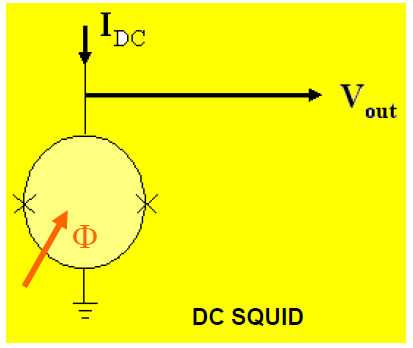
\includegraphics[width=0.5\textwidth]{./SC_figures/DC_SQUID.PNG}
\end{figure}

\item[DC SQUID] consists of two Josephson junctions that are connected by a superconducting loop. We interface with the SQUID by inputting a current into the loop or applying a magnetic field perpendicular to the loop crosssection. 

\item[Josephson junction analogue] One can think of a Josephson junction as a non-linear inductance which accumulates magnetic field energy when a current passes through it. However, the accumulated energy is not expressed in the magnetic field. It is rather thought of as the Josephson energy. 


\item[Measurement of DC SQUID] is done by applying an external current $I_b$ into the SQUID (see figure). This is also called the \emph{measurement current}. We measure the voltage over the entire SQUID by comparing the output voltage $V_{out}$ to ground. 

\item[Measured critical current] is $2I_c$, where $I_c$ is the critical current of one single junction. Since we have two junction, and the electrons have two paths to choose from, we can achieve double the critical current before superconductivity breaks down. 

\item[Circulating supercurrent] will be given by 
\beq
J = \frac{\phi_{ext}}{L}
\eeq
where $L$ is the inductance of the Josephson junction. 

\item[Current in the junctions] is given by 
\beq
I_{net} = \frac{I_b}{2} \pm J
\eeq
depending on which way the magnetic flux comes in. 

\item[$I_c$ flux dependence] is as follows:  as we increase $\phi$, $I_c$ decreases until we hit $\frac{1}{2} \phi_0$. Then it becomes more energetically favourable to change the direction of the supercurrent, after which $I_c$ starts to increase again. 

Note: I recall Ed saying that this was a fairly handwavy argument... 

The reason for the $\frac{1}{2} \phi_0$ increase is because we gain $\frac{1}{2} \phi_0$ from the supercurrent and $\frac{1}{2} \phi_0$ from the measurement current. At all times, the flux in the loop remains quantised. 

\item[Maximum flux sensitivity] is achieved by maximising the largest possible modulation of the SQUID current. Requirements:
\begin{itemize}
\item Loop inductance $L$ \emph{as small as possible}
\item $J$ as large as possible
\item Screening parameter condition
\beq
\beta_L  = 2 \frac{LI_c}{\phi_0} \leq 1
\eeq
\end{itemize}


\item[Screening parameter] written $\beta_L$ is related to the hysteresis of the SQUID. 

Question: I don't yet know in which way. 

\item[Geometric loop inductance] $L$ generally scales with the circumference of the loop. Thus we often strive to increase the effective area of the SQUID. 


\item[Measuring magnetic flux] can be done by fixing the current, usually just above $2I_c$ and measuring the change in voltage $V$. The voltage will oscillate as a function of $\phi$. Note the hyesteretic behaviour in the graph below. 

\begin{figure}[h]
  \caption{Constant current dependence.}
  \centering
    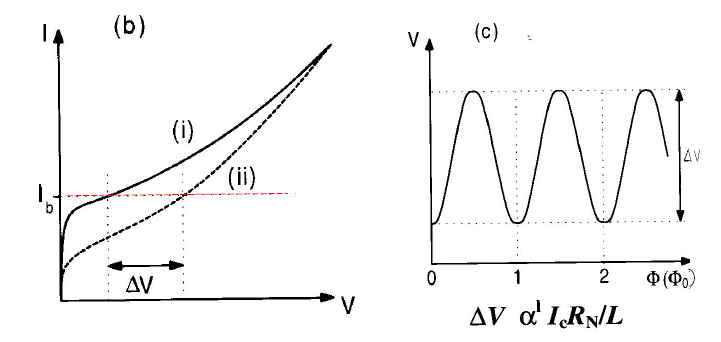
\includegraphics[width=\textwidth]{./SC_figures/Constant_Current_Measurement.PNG}
\end{figure}

The Voltage amplitude $\Delta V$ depends on how we set the external measurement current $I_B$. We want to hit the largest $\Delta V$ so that the oscillations are large. Then we obtain very fine readings for the magnetic flux. 

\item[Relative flux sensor] Because of the periodicity, the squid cannot sense absolute magnetic field, just changes in magnetic field strength. 

\item[Voltage modulation depth] $\Delta V$ is roughly given by 
\beq
\Delta V \sim \frac{I_c R_N}{1 + \beta_L}
\eeq
where $R_N$ is the junction normal resistance. For the ideal $\Delta V$, we require, 
\beq
\beta_L \leq 1
\eeq

\item[Switching voltage] is given by 
\beq
V_{switch} = I_c R_N
\eeq
Its maximum value is $\frac{1}{\Delta}$ where $\Delta$ is the energy gap of the superconductor. 

\item[Small signal mode] is an operational mode of the SQUID where we measure $\phi \ll \phi_0$. It is also known as the \emph{voltage state}. The procedure is as follows:
\begin{itemize}
\item Tune $I_b$ to maximise $\Delta V$
\item Add a fixed $B$ field to sit at a steep part of the curve, e.g. $\frac{\phi_0}{4}$
\item Measure the transfer function $\delta V = V_\phi \delta \phi$ where
\beq
V_\phi = \frac{d V}{d\phi} \bigg|{max} \sim \frac{R_N}{L}
\eeq
\item Obtain change  $\delta \phi$ in external flux
\end{itemize}



Question: What exactly is the switching voltage? 



\item[Noise in voltage state] sets the sensitivity of the SQUID. At most frequencies, the limitation is thermal (Johnson) noise. At lower frequencies, the sensitivity is limited by $1/f$ noise. All frequencies suffer white noise. 

\item[Johnson-Nyquist noise] is the electric noise generated by the thermal movement of electrons inside a conductor. The derivation of this noise is called the fluctuation-dissipation theorem. 

The total amount of thermal noise measured across a resistor depends on the measurement bandwidth $\Delta f$ of the instrument. 

\item[$1/f$ noise] also called pink noise where the frequency spectrum has a power spectral density that is inversely proportional to the frequency of the signal. 

\item[White noise] is a random signal with a constant power spectral density. 

\item[Power spectral density] is the mean square voltage per unit bandwidth. That is
\beq
\frac{V^2}{Hz}
\eeq

\item[Theoretical minimum power spectral density] for a SQUID has through simulations been found to be
\beq
S_V(f) \sim 16 k_B T R_N
\eeq
at the small signal operating point. 

\item[Flux noise] the power spectral density of the equivalent flux noise is given by 
\beq
S_\phi(f) \frac{\sim S_V(f)}{V^2 _\phi} \simeq \frac{16 k_B TL^2}{R_N}
\eeq

\item[Maximising sensitivity of the SQUID] is done by minimising $S_\phi(f)$. This is done by 
\begin{itemize}
\item Low $L$
\item Low $T$
\item High $R_N$
\item Making sure other electronics are not interfering
\end{itemize}
Note that the increase in $R_N$ will be compensated by the increase in $V^2_\phi$. 


\item[Flux locked loop] shifts the signal frequency to around a high frequency carrier. Instead of trying to measure the absolute frequency,  we modulate it by a carrier. This method is useful when we wish to measure small modulations, e.g. a small signal in the background of the Earth's magnetic field. 

\item[Measuring small fields] We increase sensitivity to \emph{flux measurements} by increasing the loop area $A$. However, changes in magnetic field are given by 
\beq
\delta B = \frac{\delta \phi}{A}
\eeq
Thus large $A$ will decrease the sensitivity. 

\item[Increasing catchment area] by coupling the SQUID to a much larger pick-up loop. This is known as a SQUID magnetometer. This way, we keep the area of the loop small while still collecting a lot of magnetic field. For this to work, the entire coupled loop must be superconducting. 

\item[Inductively coupled magnetometer] is a SQUID inductively coupled to a pickup loop via a multiturn input coil. This matches the inductance of the input coil and the SQUID. 


\item[SQUID Gradiometer] used to remove any background interference from large fields. Uses two rings where the difference in field lines will be due to their more rapid divergence, which means their source lies closer. 

\begin{figure}[h]
  \caption{SQUID Gradiometer.}
  \centering
    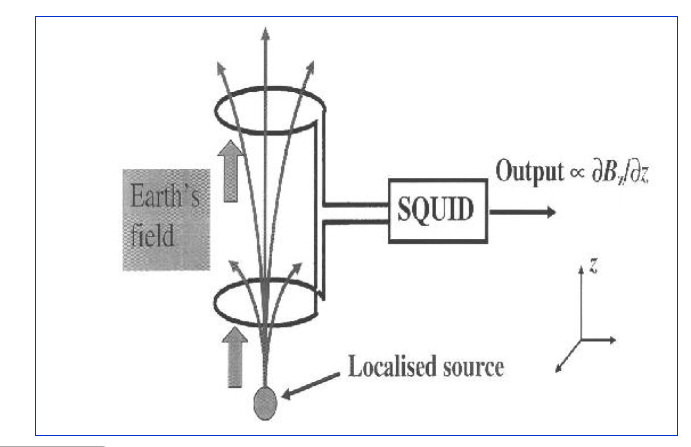
\includegraphics[width=\textwidth]{./SC_figures/SQUID_Gradiometer.PNG}
\end{figure}


\item[RF SQUID] an RF SQUID is less sensitive compared to a DC SQUID but is cheaper and easier to manufacture in smaller quantities. The consist of a single Josephson junction in a loop measured indirectly by an RF antennae. 


\begin{figure}[h]
  \caption{RF SQUID.}
  \centering
    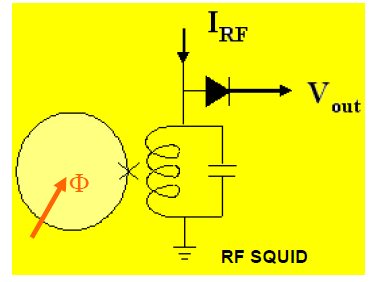
\includegraphics[width=\textwidth]{./SC_figures/RF_SQUID.PNG}
\end{figure}

\item[SQUID loop behaviour] We have both flux quantisation in the loop and phase change $\delta $ around the junction. They are thus related by 
\beq
\delta  + 2 \pi \frac{\phi_T}{\phi_0} = 2 n \pi
\eeq
where $\phi_T$ is the total flux in the loop. 

The total flux $\phi_T$ is made up of the applied flux $\phi_a$ and the flux induced by the screening current, 
\beq
J = I _0 \sin{\delta}
\eeq
This leads to a relation
\beq
\phi_T = \phi_a - LI_0 \sin{\left( 2\pi \frac{\phi_T}{\phi_0} \right)}
\eeq
which can be either single valued or hysteretic. 

Question: How is this derived? Where does the inductance $L$ come into the picture? 

Attempt at answer: Probably because we have the relation
\beq
L = \frac{\phi}{I}
\eeq
That is, the inductance is a measure of how much flux links a circuit when a current flows. 

\item[RF SQUID parameter] determines whether an RF SQUID is hysteretic or not. It is written
\beq
\beta_{rf} =  \frac{2\pi LI_0}{\phi_0}
\eeq


\item[RF SQUID readout] is done as follows:
\begin{itemize}
\item Couple the loop with the Josephson junction to an LCR oscillator circuit 
\item Drive LCR circuit close to its resonance by n RF current
\item Measure the voltage oscillation of LCR circuit 
\end{itemize}

Question: I am unsure about the last step - it is not clear from the notes. 

\item[Dissipative regime] in this mode, the SQUID makes transitions between quantum states. It dissipates energy at a rate that is periodic in $\phi_a$. This modulates the $Q$ values of the LCR circuit. As a result, the RF voltage output $V_{out}$ is periodic in $\phi_A$. 



\item[Dispersive regime] (not to be confused with the above!) in this non-hysteretic regime the RF SQUID behaves as a flux sensitive inductor. The inductance is linked to an emf, through
\beq
E = - \frac{d \phi}{dt} = - L \frac{d\phi}{dt}
\eeq
Question: Something is wrong here. I have never seen Faraday's law with $L$ in it. 

Given the Josephson equations, 
\beq
I = I_c \sin{\phi}
\eeq
\beq
\frac{d\phi}{dt} = \frac{2e}{\hbar} V
\eeq
We can relate the Josephson current to an inductance
\beq
L_J = \frac{\phi_0}{2 \pi I_c \cos{\phi}}
\eeq

And we obtain
\beq
L = \frac{\phi_0}{2 \pi I_c \cos{\phi}}
\eeq
Note that this makes the inductance non-linear. 

Question: Derivation? 

\item[Dissipative mode readout] the RF SQUID is read out by detecting the change in the Josephson junction. This is done by observing the change in $Q$ due to the flux change. 



\end{description}

\section{John Fenton's Lectures - Three parts}
\subsection{Quantised Josephson junctions}
This is the quantum part about the junctions. 

\begin{description}
\item[Potentials] We can think of the bumps in the washboard model as 1D potentials. Treat the electron as a harmonic oscillator and find energy levels (for a single mode)
\beq
E_n = \hbar \omega_0 \left(  n + \frac{1}{2} \right)
\eeq

\item[Potentials in Josephson junction] Potential is not harmonic but \emph{anharmonic} - energy levels are not spaced evenly. It can be estimated by 
\beq
U(\phi) = - \frac{h}{2e} I \phi - E_J \cos{\phi}
\eeq
Note a static part (which depends on the external current $I$) and an oscillating part. 

\item[Analogues for the washboard] are
\begin{itemize}
\item Tilt of washboard = external current bias $I$
\item Bump amplitude = Josephson energy $E_J$
\item Bump periodicity = phase difference $\phi = \phi_1 - \phi_2$
\end{itemize}

\item[Lifetime of electron in potential] is limited due to the electron quantum tunnelling out of the potential. 

\item[Voltage state] means when the electron escapes the potential, and `starts rolling' without stopping in an undamped system. 

\item[Consequence of tunnelling] means that even as we go to 0 K, we see occasional current and voltage spikes once an electron manages to tunnel out. 

\item[Irradiation of microwaves] increases the tunnel rate. 

Question: Exactly which mechanism induces this? There are only graphs in the notes... :(

\item[Josephson junction Hamiltonian ] for zero current bias given by 
\beq
H = U(\phi) + 4 E_c N^2 = U(\phi) - 4 E_c \frac{\p ^2}{\p \phi ^2}
\eeq
where
\beq
N = - i \frac{\p}{\p \phi}
\eeq
and
\beq
E_c = \frac{e^2}{2C}
\eeq
Question: Is this the conductance of the junction, or the combination addition of all capacitances in the circuit? 

Attempt at answer: I think it is only the junction. In the notes, the capacitance is used as an analogy of the `ball's mass'. 

Note that $\phi$ and $N$ are \emph{conjugate variables} - they are not simultaneously observable. 

Question: Why do we have a $N^2$ term here? I haven't really seen those around before. 




\item[$E_J \gg 	E_c$ regime] will see the wavefunction $\psi(\phi)$ sharply peaked around specified $\phi$. It implies
\begin{itemize}
\item Small $\delta \phi$ = $\phi$ well defined
\item Large $\Delta N$ = $N$ not well defined
\end{itemize}


Question: Which wavefunction are we considering? The total wavefunction of both superconductors, or just one of them? 

\item[$E_J \ll E_c$ regime] wavefunction $\psi(\phi)$ varies slowly over  some range. 
\begin{itemize}
\item Large $\Delta \phi$ = $\phi$ not well defined
\item Large $\Delta N$ = $N$ well defined
\end{itemize}
I believe that these assertions come from when we would average over many turns of the wavefunction. 

\item[Deriving the Josephson Equations from the Schrodinger equation] can be done by realising that tunnelling changes the number of Cooper pairs on one junction electrode, $N \rightarrow N + 1$. This warrants the Hamiltonian
\beq
H_J = - \frac{E_J}{2} \sum_{- \infty}^\infty \left( \ket{N} \bra{N+1} + \ket{N+1} \bra{N} \right)
\eeq
From this we can solve the Schrodinger equation as well as prove the complementarity of $N$ and $\phi$

\end{description}

\subsection{Qubits form Josephson junctions}
\begin{description}
\item[Motivation] advantages and disadvantages are:
\begin{itemize}
\item Good for scaling
\item Easy to couple 
\item Couples too easily to environment
\item Short coherence times
\end{itemize}

\item[Josephson junction qubits] come in three varieties:
\begin{itemize}
\item Charge qubits
\item Flux qubits
\item Phase qubits
\end{itemize}


\item[Qubit requirements] are tunable separation between energy levels. 


\item[Phase qubits] is a current-biased Josephson junction, operated in the zero voltage state with a non-zero current bias. 

The \emph{energy levels} are found in local minima of the washboard potential. 

We \emph{manipulate} the qubit by adding microwave pulses which cause Rabi oscillations. 

\begin{figure}[h]
  \caption{Phase qubit.}
  \centering
    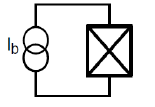
\includegraphics[width=\textwidth]{./SC_figures/Phase_Qubit.PNG}
\end{figure}

Question: What does the box around the function mean? That we are in the zero voltage state? 

\item[Flux qubits] are Josephson junctions which will have a persistent current flowing continuously as external flux is applied. They are based on RF SQUIDS. 

The qubit states are defined by direction of the circulating currents. We make use of the flux quantum to treat it as a qubit. When the external flux reaches $\frac{1}{2}\phi_0$ the two current energy levels are close together, which enables qubit operation. 

\item[Potential for RF SQUID] is given by
\beq
U(\phi_T) = - E_J \cos{\left( \frac{2\pi \phi_T}{\phi_0} \right)} + \frac{(\phi_T - \phi_{ext} )^2}{2L}
\eeq
This potential always has two minima, like the wine-bottle potential. We can shift this potential intro three modes:
\begin{itemize}
\item $\phi_{ext} < \frac{\phi_0}{2} $ gives low left potential and high right potential
\item $\phi_{ext} = \frac{\phi_0}{2}$ gives two equally deep potential
\item $\phi_{ext} > \frac{\phi_0}{2}$ gives a high left potential and low right potential
\end{itemize}


\item[Consequence of double minima] there is tunnelling between the two minima, which hybridises the states of the potential wells. This causes them to move apart in energy. 	We can use this to sit ourselves at $\phi_{ext} = \frac{\phi_0}{2}$, then tunnelling causes there to e a ground state and an excited state. The ground state has a symmetric wavefunction while the excited state has an antisymmetric wavefunction. 

Question: Exactly how is the degeneracy broken if we have tunnelling? 


\item[Flux qubit readout] can be done by inductively couple the qubit to a neighbouring circuit. Then the current flow in the flux can be read out. 

\item[Coupling flux qubits] can be done by invoking a flux coupling. This means that the state of one qubit will be altered by the state of the second qubit. Through this, we can invoke a CNOT gae. 

Question: It is not clear how the coupling is performed. 

\item[Charge qubits] the basis states of a charge qubit are charge state, representing the presence or absence of Cooper pairs. A charge qubit is formed by a a tiny superconducting island (known as a Cooper-pair box) coupled by a Josephson junction to a superconducting reservoir. 

The potential is given by 
\beq
E = - E_J \cos{\phi}   + 4 E_c (N - N_g)^2
\eeq

Central to the setup is a Cooper pair box, it consists of an island the charge states of which it involves a macroscopic number of conduction electrons. 

Readout is done by electrostatically coupling the island to an extremely sensitive electrometer. 

\item[Coupling between qubits]  can be done by
\begin{itemize}
\item Flux qubits are coupled with an inductive coupling
\item Charge qubits are coupled using a capacitive coupling
\end{itemize}

\end{description}

\subsection{Metrological applications of superconducting currents}
\begin{description}
\item[screw this]

\end{description}

\end{document}